%! TeX program = lualatex
\documentclass[a4paper,11pt]{article} 
% packages
\usepackage{censor}
\StopCensoring
\usepackage{fontspec}
\setmainfont{EB Garamond}
% for tironian et fallback
% % \directlua{luaotfload.add_fallback
% % ("emojifallback",
% %      {"Noto Serif:mode=harf"}
% % )}
% % \setmainfont{EB Garamond}[RawFeature={fallback=emojifallback}]

\setmonofont[Scale=MatchLowercase]{Deja Vu Sans Mono}
\usepackage[a4paper,left=2cm,right=2cm,top=\dimexpr15mm+1.5\baselineskip,bottom=2cm]{geometry}
\setlength{\parindent}{0pt}

\usepackage{fancyhdr}       % Headers and footers 
\fancyhead[R]{\normalfont \leftmark}
\fancyhead[L]{}
\pagestyle{fancy}

\usepackage{microtype}      % Slightly tweak font spacing for aesthetics
\usepackage[english]{babel} % Language hyphenation and typographical rules
\usepackage{xcolor}
\definecolor{linkblue}{RGB}{0, 64, 128}
\usepackage[final, colorlinks = false, urlcolor = linkblue]{hyperref} 
% \newcommand{\secref}[1]{\textbf{§~\nameref{#1}}}
\newcommand{\secref}[1]{\textbf{§\ref{#1}~\nameref{#1}}}

\usepackage{pgfgantt}
\usepackage{changepage}     % adjust margins on the fly
\usepackage[sorting=none, backend=biber, style=numeric, date=iso, urldate=iso]{biblatex}
\addbibresource{references.bib}

\usepackage{minted}
\usemintedstyle{algol_nu}

\usepackage{pgfplots}
\pgfplotsset{width=\textwidth,compat=1.9}

\usepackage{caption}
\newenvironment{code}{\captionsetup{type=listing}}{}
\captionsetup[listing]{skip=0pt}
\setlength{\abovecaptionskip}{5pt}
\setlength{\belowcaptionskip}{5pt}

\usepackage[yyyymmdd]{datetime}
\renewcommand{\dateseparator}{--}

\usepackage{enumitem}

\usepackage{titlesec}

\author{Andrew Hayes}
\newcommand{\sectionbreak}{\clearpage}

\begin{document}
\begin{titlepage}
    \begin{center}
        \hrule
        \vspace*{0.6cm}
        \Huge \textsc{ct413}
        \vspace*{0.6cm}
        \hrule
        \LARGE
       \vspace{0.5cm}
       Project Definition Document
       \vspace{0.5cm}
       \hrule
       \vfill
       \centering
       
\includegraphics[width=0.80\textwidth]{./images/University_Of_Galway_Logo__Positive_Portrait.png}
       \vfill
       \hrule
        \begin{minipage}{0.495\textwidth} 
            \vspace{0.4em}
            \raggedright
            \normalsize 
            \begin{tabular}{@{}l l}
                Name: & Andrew Hayes \\
                Student ID: & 21321503 \\
                % E-mail: & \href{mailto://a.hayes18@universityofgalway.ie}{a.hayes18@universityofgalway.ie} \\
                Programme: & 4BCT
            \end{tabular}
        \end{minipage}
        \begin{minipage}{0.495\textwidth} 
            \raggedleft
            \vspace*{0.8cm}
            \Large
            \today
            \vspace*{0.6cm}
        \end{minipage}
        \medskip\hrule 
    \end{center}
\end{titlepage}

\pagenumbering{roman}
\newpage
\tableofcontents
\newpage
\setcounter{page}{1}
\pagenumbering{arabic}

\section{Project Overview}
\subsection{Introduction}
The purpose of this project is to create a useful \& user-friendly application that can be used to track the current whereabouts \& punctuality of various forms of Irish public transport, as well as access historical data on the punctuality of these forms of transport.
In particular, this location-tracking is to take the form of a live map upon which every currently active public transport service is plotted according to its current location, with relevant information about these services and filtering options available to the user.
\\\\
The need for this project comes from the fact that there is no extant solution for a commuter in Ireland to track the current location and whereabouts of all the different public transport services available to them.
There are some fragmented services that purport to display the live location of one particular mode of transport, such as the Irish Rail live map\supercite{liveir}, but this can be slow to update, displays limited information about the services, and only provides information about one form of public transport.
\\\\
The need for an application that tracks the live location \& punctuality of buses in particular is felt here in Galway, especially amongst students, as the ongoing housing shortage drives students to live further \& further away from the university and commute in, with Galway buses often being notoriously unreliable and in some cases not even showing up, many commuters could benefit from an application that tells them where their bus actually is, not where it's supposed to be.
In fact, the 411 bus route here in Galway is so notorious for being a ``ghost bus'' that never seems to show up that a local band wrote a song about the route that has received over 18,000 listens on Spotify\supercite{411}!

\subsection{Tools \& Software}
\subsubsection{Development Tools}
\begin{itemize}
    \item   The front-end development will be done in the JavaScript-based web-development framework \textbf{React}\supercite{react}, with a view to making the code written as portable as possible to \textbf{React Native}\supercite{native}, a development framework based on React for making native applications for the web, Android, and iOS.
        React was chosen for its popularity and the wide array of libraries \& plug-ins that it supports, as well as the fact that it can be easily be adapted to React Native to support native mobile applications.
        \\\\
        It was decided that development would be focused on React as opposed to React Native, as React Native development is more restrictive with the libraries \& features it supports, and native app development requires a greater degree of platform-specific domain knowledge \& development which could greatly hamper the development of the project.

    \item   Remaining front-end development will be done using the traditional HTML, CSS, \& JavaScript.

    \item   Mapping \& plotting of transportation will be done with the \textbf{MapBox}\supercite{mapbox} platform, which was chosen for its integration to React \& React Native, as well as its generous free API tier.
            The map tiles will be sourced from \textbf{OpenStreetMap}\supercite{osm} as they are free-to-use \& have excellent coverage, particularly in Ireland.

    \item   Any web hosting, server-side computation, \& database storage will be done with \textbf{AWS}\supercite{aws}.
            A serverless solution was chosen for optimal scalability and to circumvent system administration \& hardware requirements inherent in self-hosting a database.
            AWS specifically as a serverless solution was chosen due to my previous professional experience with AWS, its extensive \& comprehensive documentation, and its reasonably expansive free tier.
            AWS also supports JSON-based databases, which is ideal for a web application that will be using JSON to represent its data internally anyway.

    \item   Any back-end, server-side code will be written in JavaScript, chosen for several reasons: the front-end will be in JavaScript regardless which allows for a more homogeneous codebase for easier maintenance \& re-usable tooling, JavaScript is well-supported by AWS, JavaScript has a wide array of libraries that can be used, and many API documentations are made with JavaScript development in mind. 
\end{itemize}

\subsubsection{Data Sources}
Data will be sourced from a number of public APIs and stored in a database, which both helps to prevent repeated, unnecessary calls to these APIs as the project scales as well as facilitating historical storage \& analysis of the data.
\begin{itemize}
    \item   Realtime train \& DART location data, along with station location data will be obtained from the Irish Rail Realtime API\supercite{trains}.
    \item   Realtime Luas data will be obtained from the Transport Infrastructure Ireland's Luas Forecasting API\supercite{luas}.
    \item   Realtime bus data and bus route information will be obtained from the National Transport Authority General Transport Feed Specification (GTFS) API\supercite{gtfs}.
\end{itemize}

\subsubsection{Project Management Tools}
\begin{itemize}
    \item   All software development will be managed using the version control software \textbf{Git}\supercite{git}, with the Git repository being hosted on \textbf{GitHub}\supercite{github}.
        Git is a near-ubiquitous choice for version control software, and I have professional experience both with Git \& GitHub.
        GitHub also has excellent support for CI/CD pipelines via \textbf{GitHub Actions}\supercite{actions}, which will be very useful if I am integrating any sort of CI/CD into my project.

    \item   Additionally, since the deliverable documents for this project are being written in {\LaTeX} and the progress notebook in Markdown, these files will be also version-controlled and backed-up using Git \& GitHub.
\end{itemize}

\subsection{Deliverables}
The following deliverables and their respective due dates have been set by the university:
\begin{itemize}
    \item   2025–01–05: Project Definition Document \& Progress Notebook;
    \item   2025–04–06: Final Project Report;
    \item   2025–04–09 – 2025–04–10: Project Demonstration \& Viva Voce.
\end{itemize}

\section{Background Research}
% Irish rail map, google maps, flight radar, dublin bus tracker.
As background research for this project, I created a list of transport-tracking applications that I could find online which I then analysed to determine what negatives they had that I could improve on and what positives they had that I could take inspiration from.

\subsection{Irish Rail Live Map}
The Irish Rail Live Map\supercite{liveir} displays the current location of Irish Rail intercity, commuter, \& DART services, with clickable icons that display information about the selected service including the lateness of the train and its next stop.
\begin{figure}[H]
    \centering
    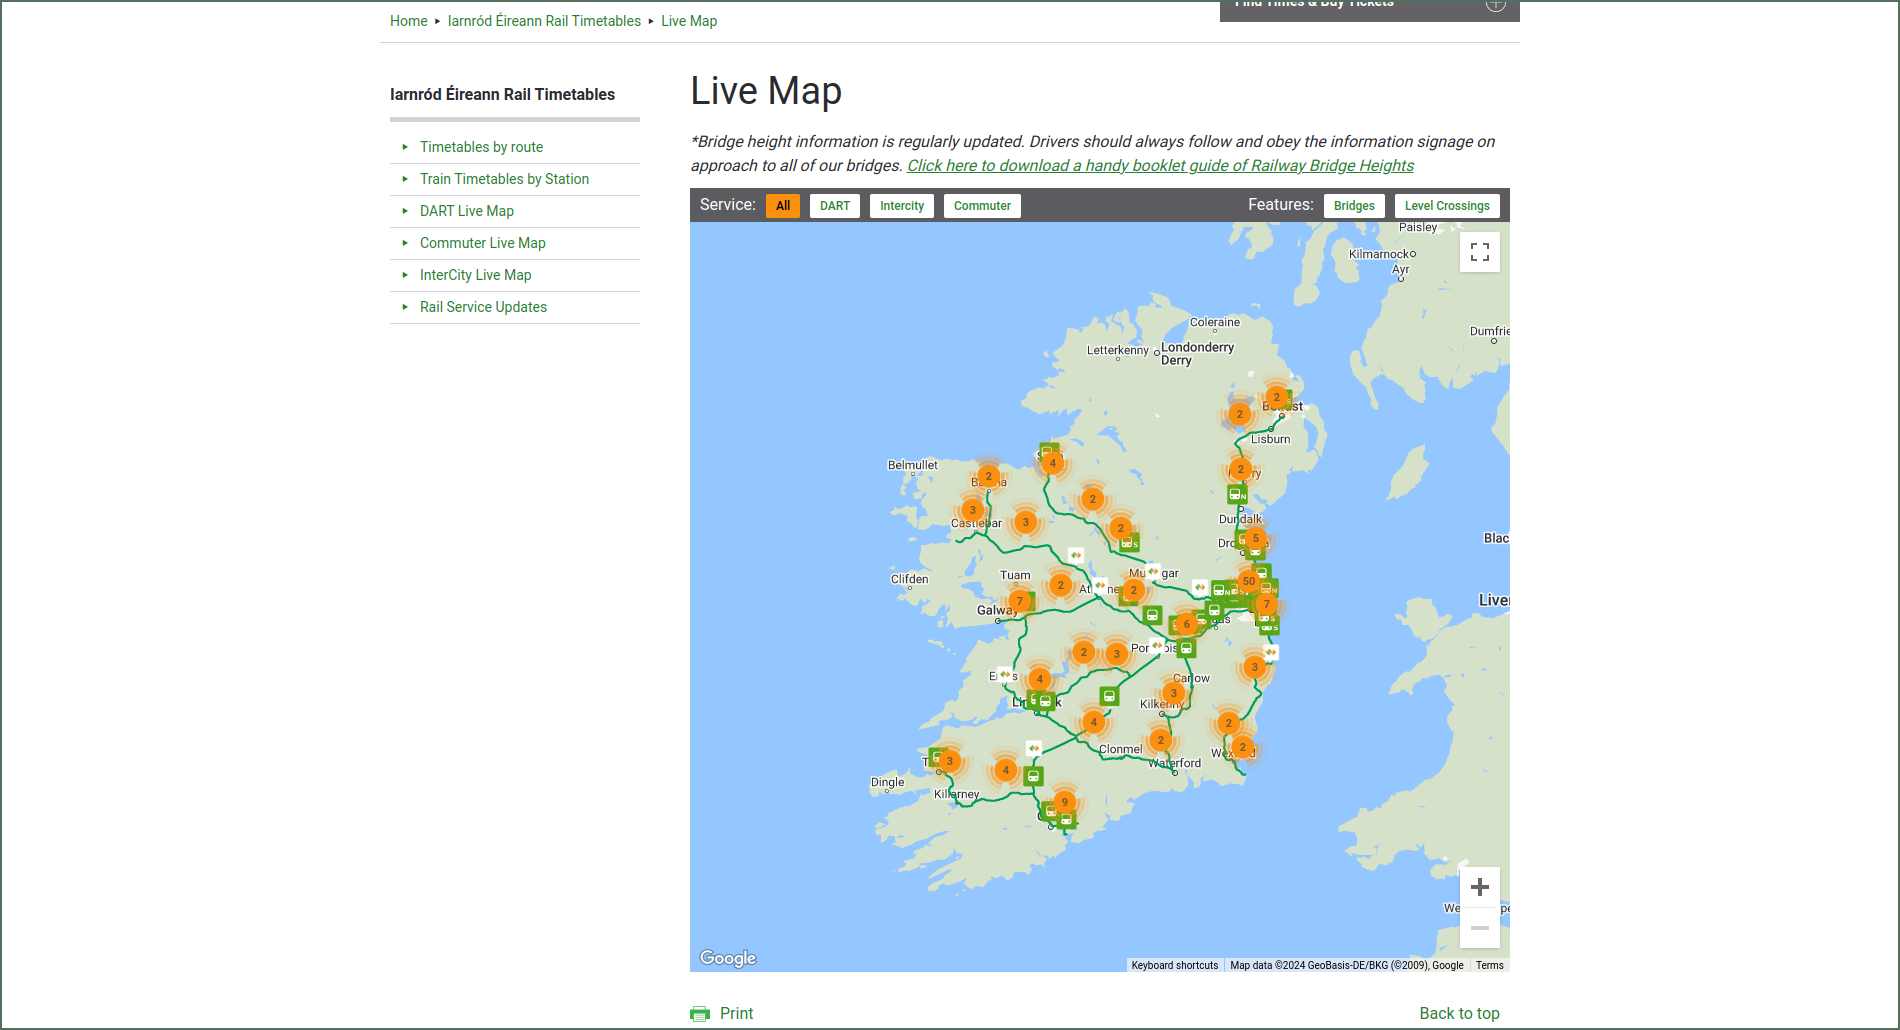
\includegraphics[width=\textwidth]{./images/irlive.png}
    \caption{Irish Rail Live Map}
\end{figure}

Strengths of the Irish Rail live map include:
\begin{itemize}
    \item   Services can be clicked on to display a pop-up panel showing the punctuality of that service, the next stop of that service, and the stops on that service's route.
    \item   There are basic filtering options to display a specific type of service such as DARTs.
    \item   Bridges, level crossings, \& stations are shown on the map.
            The stations can also be selected and information about them viewed.
\end{itemize}

Limitations of the Irish Rail live map include:
\begin{itemize}
    \item   The pop-up information panel covers the entire map and hides it.
    \item   There is no search feature to find a specific service.
    \item   The filtering options are greatly limited.
    \item   The UI is slow and not particularly responsive.
    \item   There is no visual distinction between the icons for different kinds of services.
\end{itemize}

\subsection{Google Maps}
Google Maps\supercite{gmaps} is a common choice for finding the next the upcoming nearby services and route planning.
It covers a number of different types of service, include buses \& trains.
I have included the mobile UI here alongside the desktop UI as there is no live service information on the desktop version.

\begin{minipage}{0.20\textwidth} 
\begin{figure}[H]
    \centering
    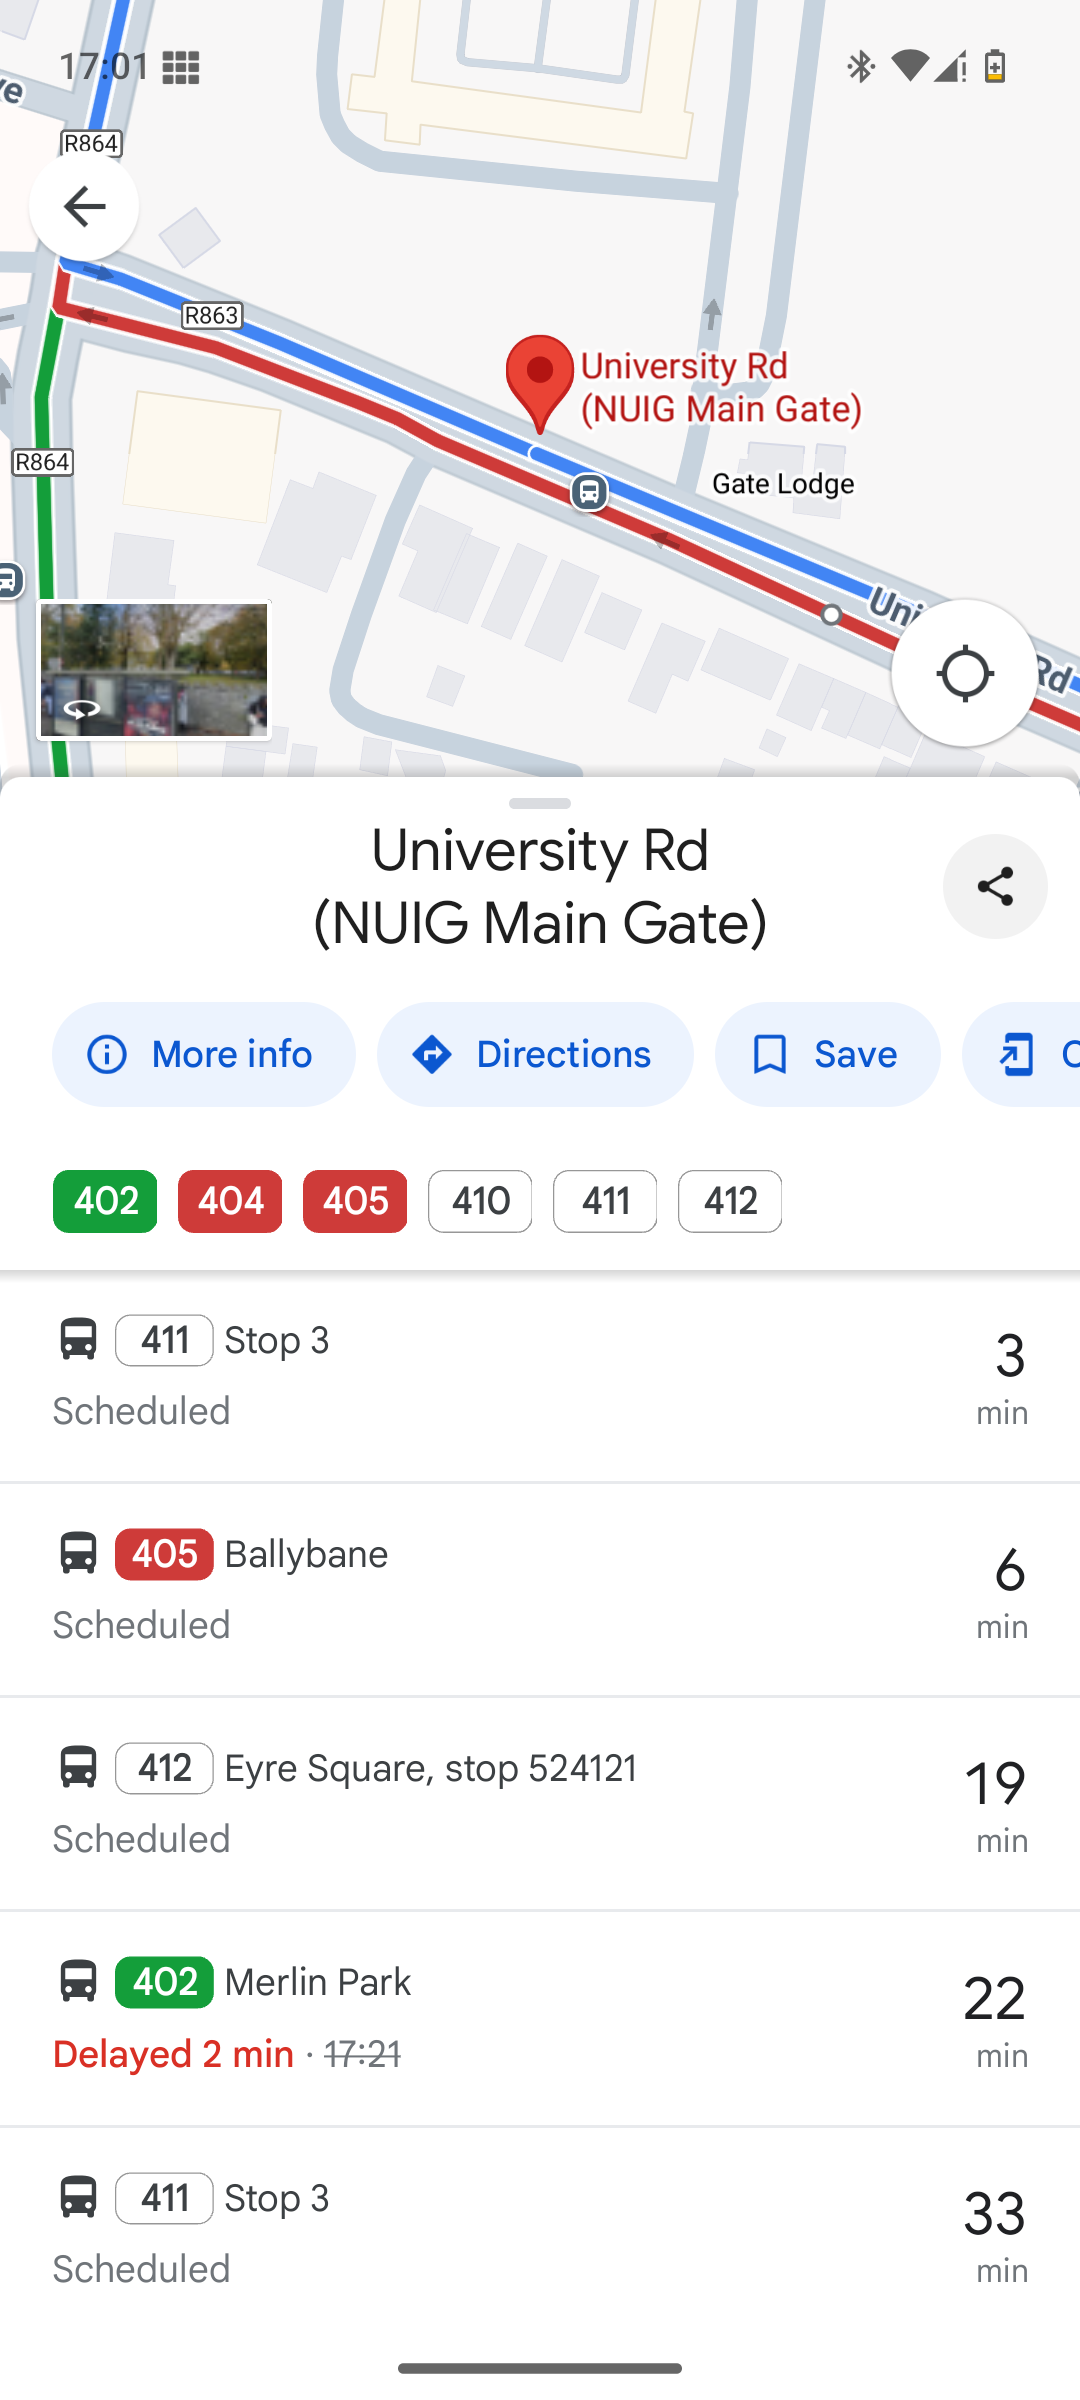
\includegraphics[width=\textwidth]{./images/gmobile.png}
    \caption{Google Maps Mobile View}
\end{figure}
\end{minipage}
\begin{minipage}{0.80\textwidth} 
\begin{figure}[H]
    \centering
    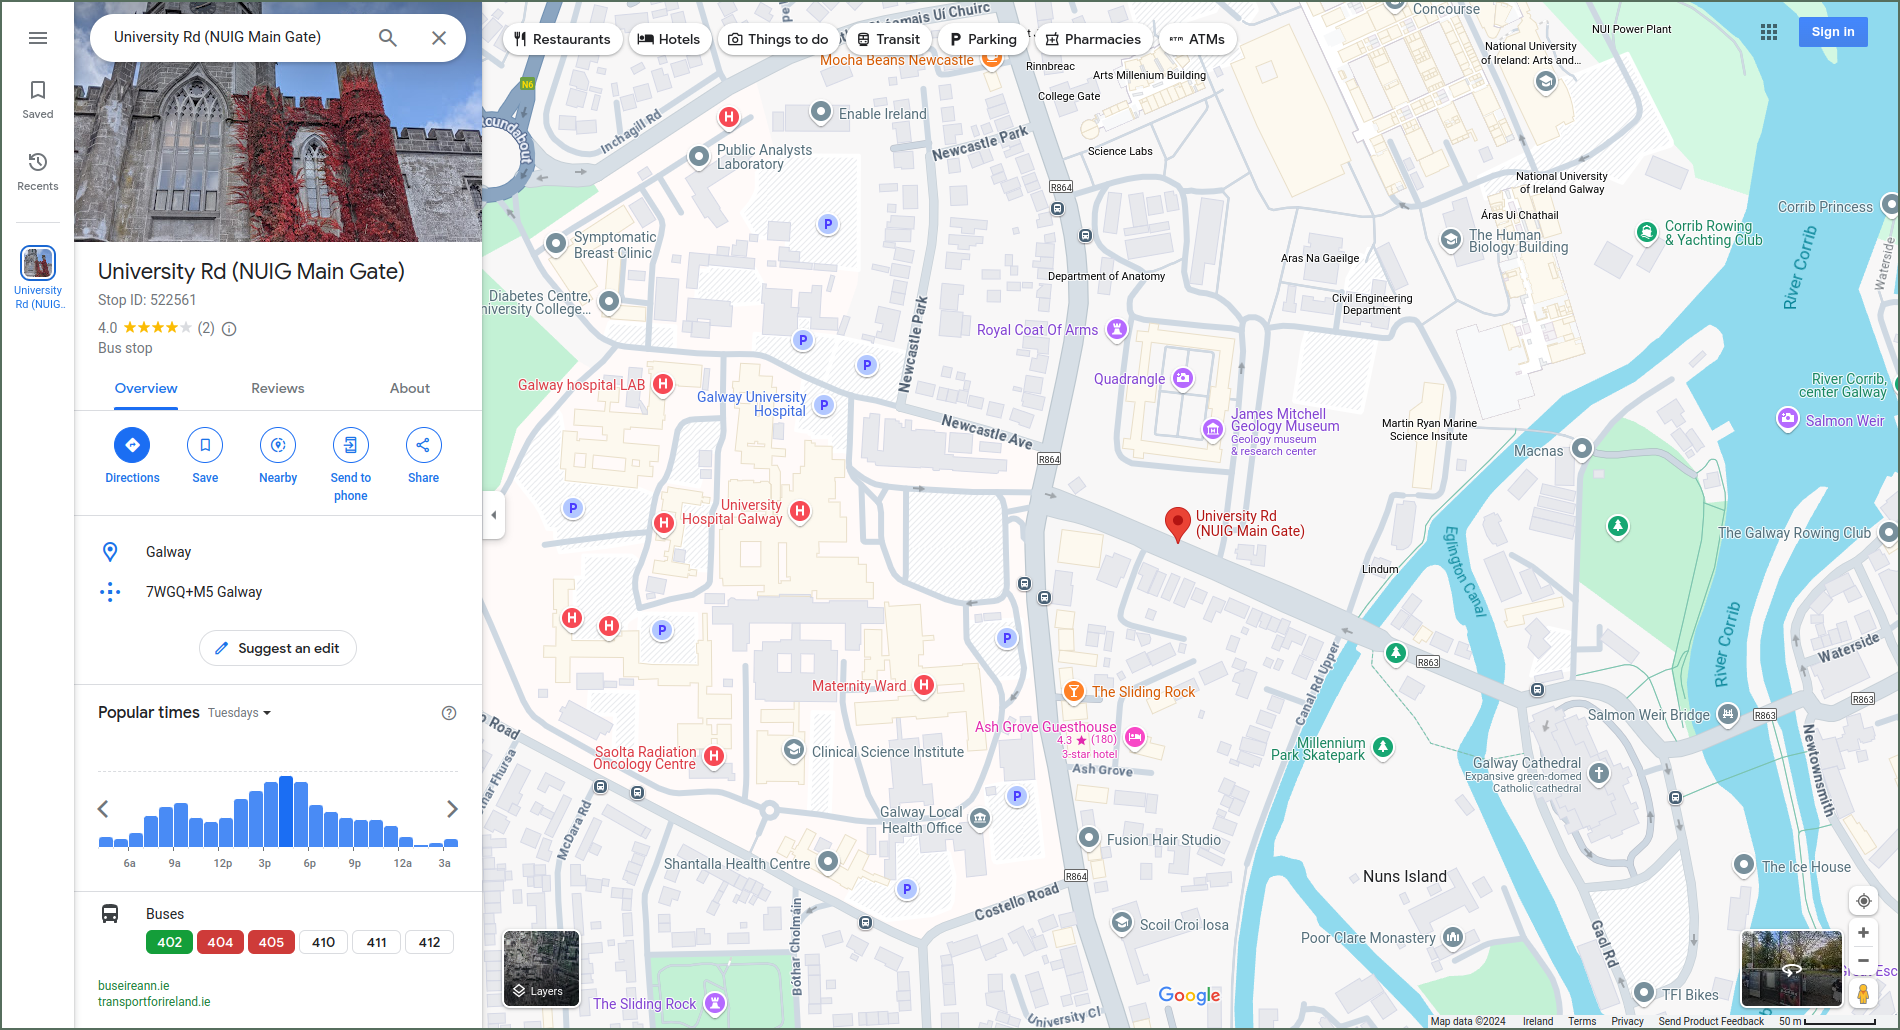
\includegraphics[width=\textwidth]{./images/gdesk.png}
    \caption{Google Maps Desktop View}
\end{figure}
\end{minipage}

Strengths of Google Maps include:
\begin{itemize}
    \item   It facilitates route determination, and can tell the user about what services they need to take to get any arbitrary location.
    \item   The mobile version lists when services are due and how long they will be delayed.
\end{itemize}

Limitations of Google Maps include:
\begin{itemize}
    \item   There is no live service information on the desktop version.
    \item   Vehicle locations are not plotted on the map and thus the user cannot tell where the service actually is.
    \item   Specific services cannot be searched for, and there is no filtering to display only a certain type of service.
\end{itemize}

\subsection{TFI Live Departures}
The TFI Live Departures map\supercite{tfilive} shows live departure information for both bus stops and train stations.
\begin{figure}[H]
    \centering
    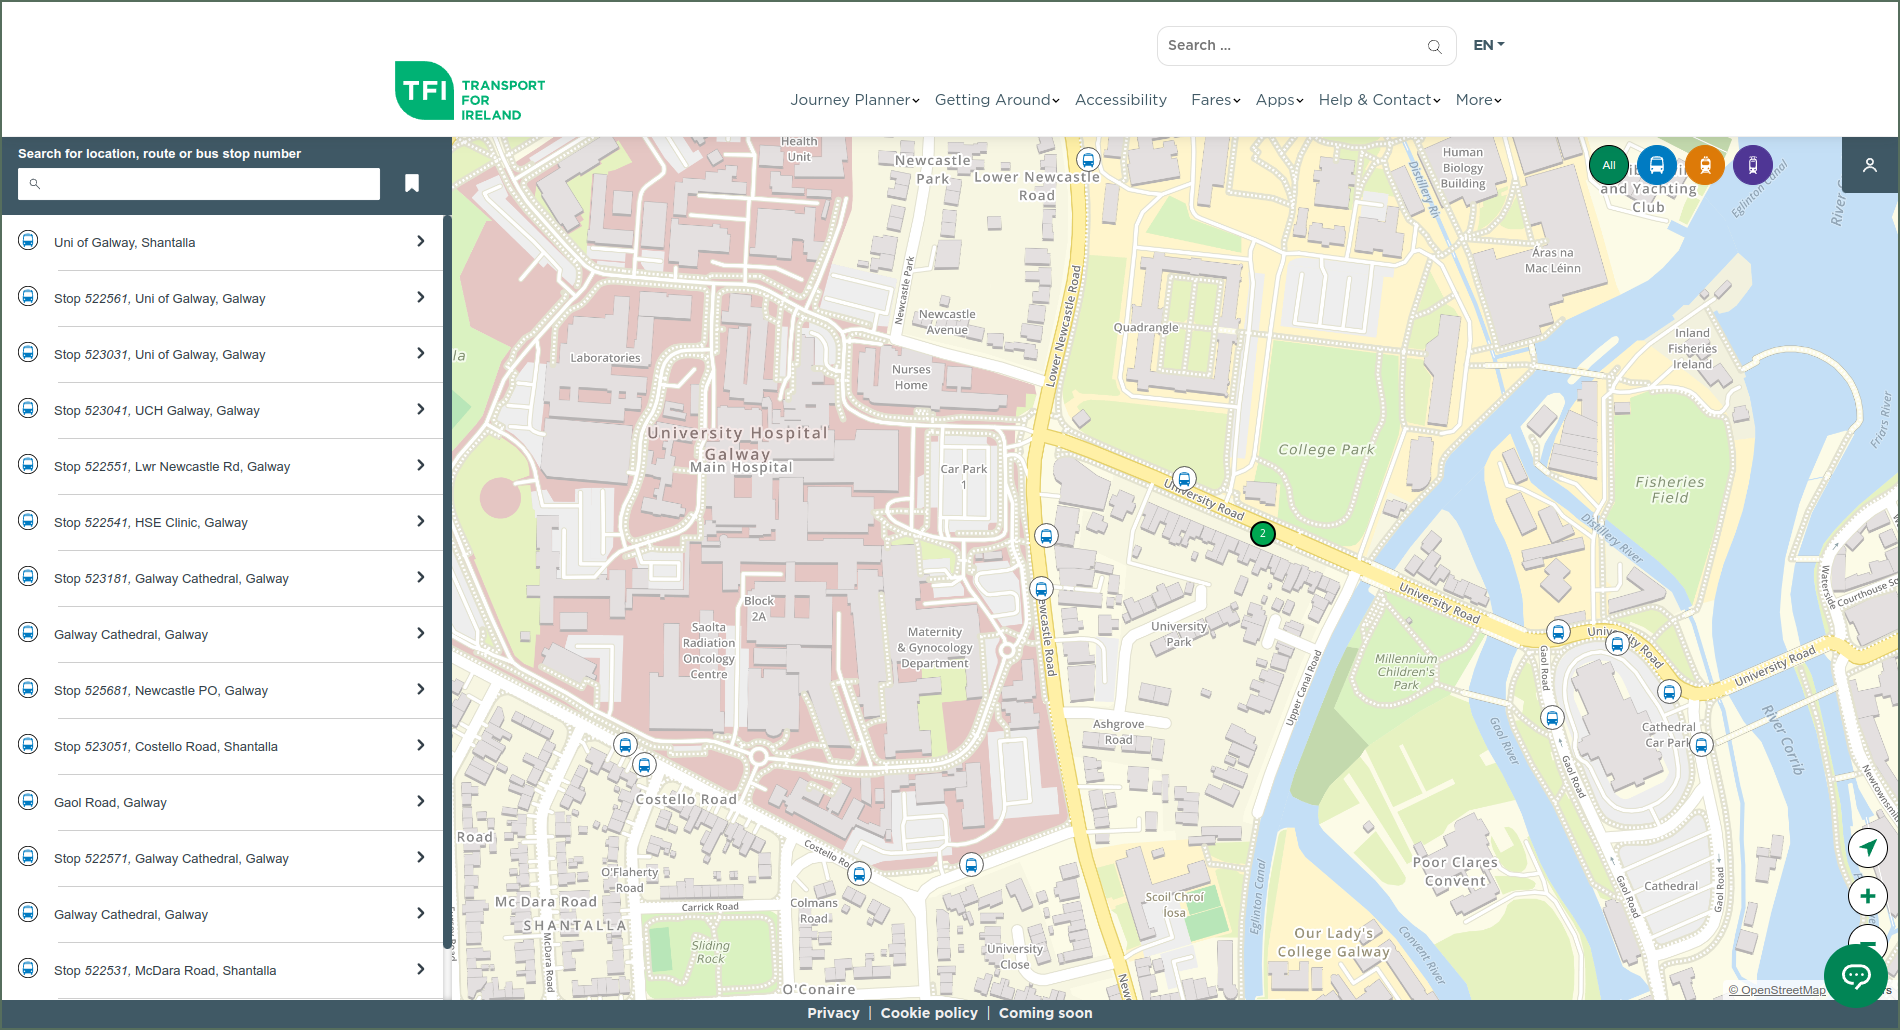
\includegraphics[width=\textwidth]{./images/tfi.png}
    \caption{TFI Live Departures Map}
\end{figure}

Strengths of the TFI Live Departures map include:
\begin{itemize}
    \item   A stop or a station can be clicked on to show a pop-up information panel that appears at the side of the screen and does not cover the map.
    \item   There is a powerful search feature that allows the user to search by location, route, or stop number.
    \item   If a specific route is selected, the route is highlighted on the map and its stops are plotted.
    \item   The map is highly detailed, making it easier to find a particular location on the map and find nearby services.
\end{itemize}

Limitations of the TFI Live Departures map include:
\begin{itemize}
    \item   The map doesn't show the live locations of the services, it shows the stops or stations from which the services depart.
    \item   The map has no filtering options beyond the search feature.
    \item   The map has to be zoomed in very far to actually display the stations in that area, which while understandable from a technical perspective, makes the map more difficult to use \& navigate.
    \item   It doesn't say whether or not services will be delayed or where they currently are, only saying when they are scheduled for.
\end{itemize}


\subsection{Flightradar24}
While Flightradar24\supercite{radar} is a live-tracking application for monitoring aeroplane \& helicopter flights which are not within the scope of this project, I nonetheless chose to include it in my analysis as I believe that it is a particularly good example of transport-tracking UI.

\begin{figure}[H]
    \centering
    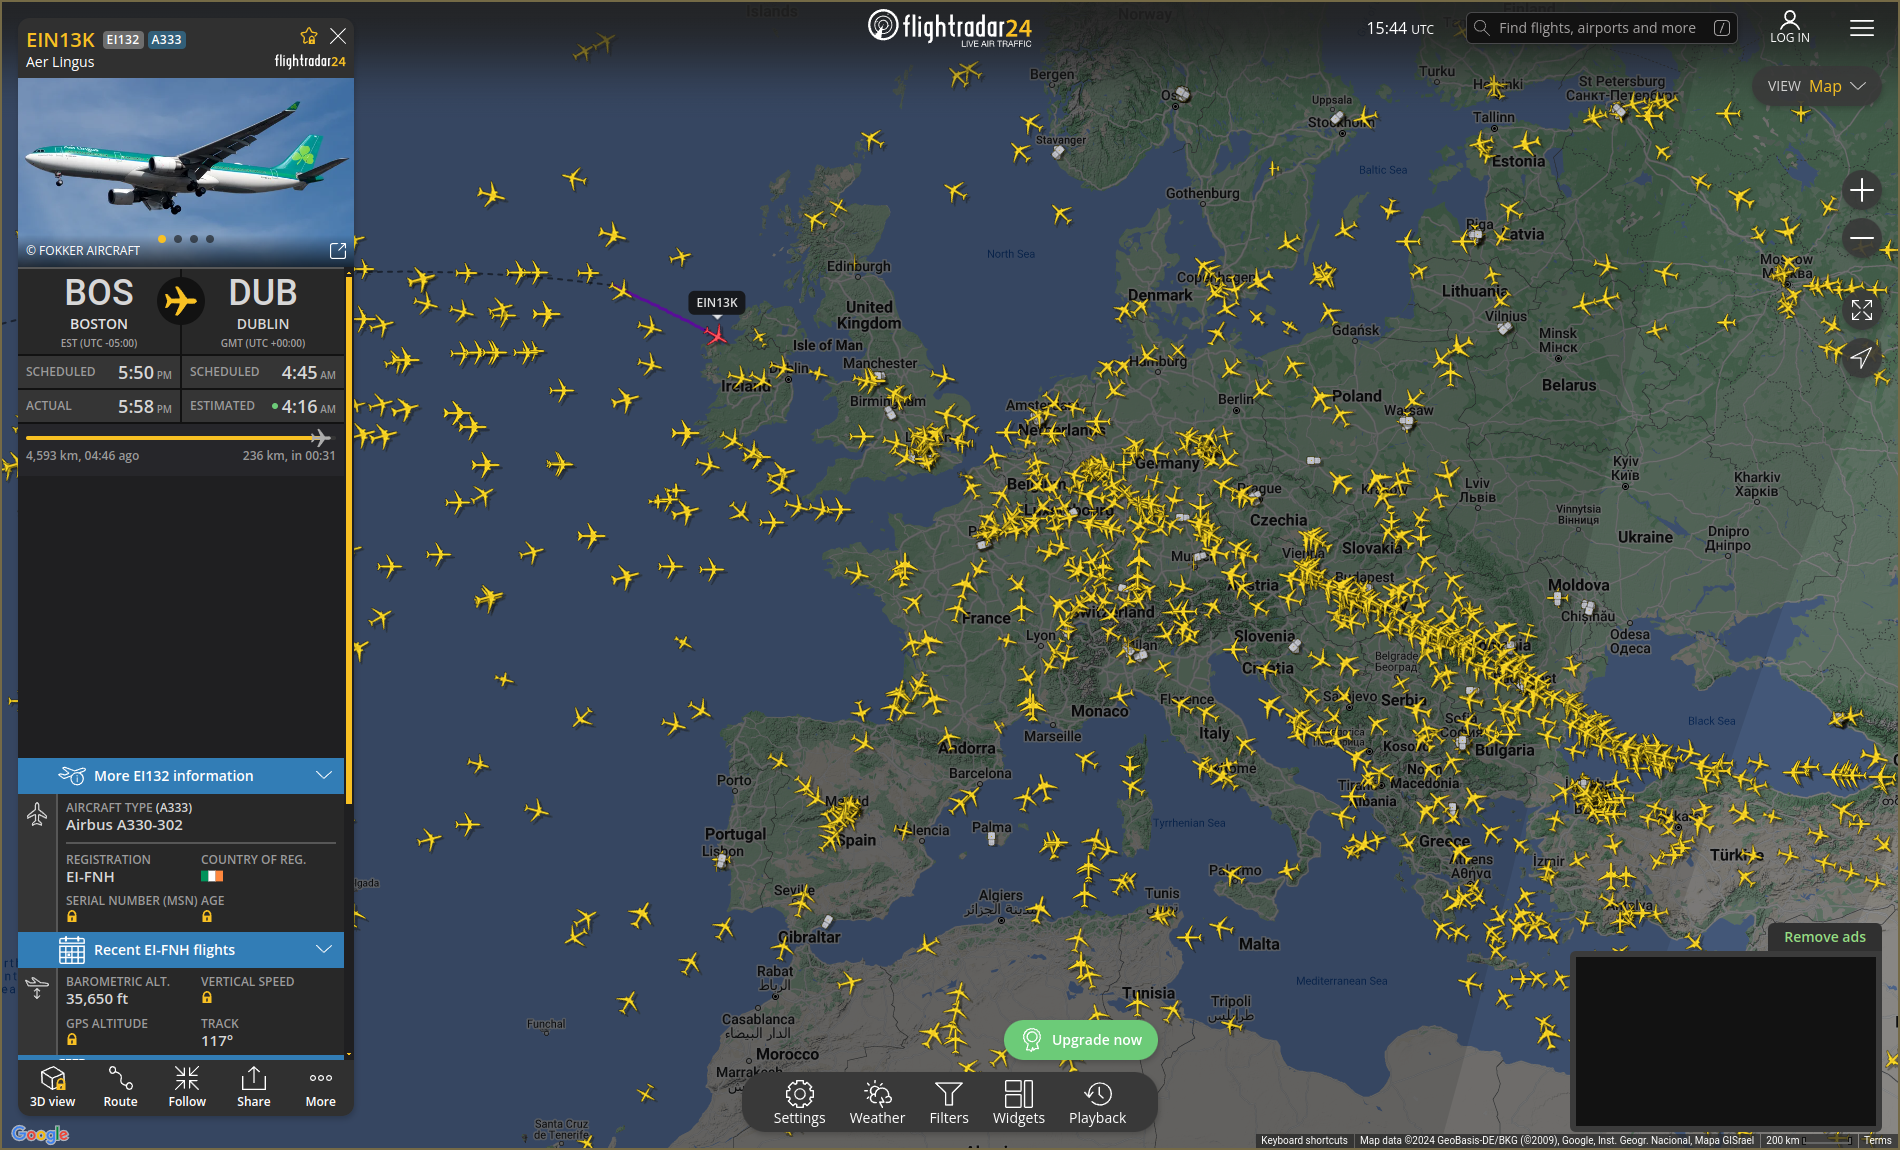
\includegraphics[width=\textwidth]{./images/flightradar.png}
    \caption{Flightradar24 UI}
\end{figure}

Strengths of Flightradar24 include:
\begin{itemize}
    \item   Ability to select a given service and open a pop-up panel that displays details about that service.
    \item   Selected services are highlighted in red on the map.
    \item   The information panel shows the scheduled departure time, the actual departure time, the scheduled arrival time, \& the estimated arrival time.
    \item   The information panel displays an image of the selected vehicle.
    \item   Searching \& filtering features.
    \item   Larger planes have larger icons on the map and helicopters have distinct icons from planes.
\end{itemize}

The few limitations I could identify are:
\begin{itemize}
    \item   Bookmarking a vehicle requires a paid account.
    \item   The UI contains advertisements for free users.
\end{itemize}

However, these are minor inconveniences and are the result of business decision rather than a design decision.





\section{Project Objectives}
\subsection{Core Objectives}
The core objectives of the project are as follows:
\begin{itemize}
    \item   Create a live map of train, DART, bus, \& Luas services in Ireland, which displays the real-time whereabouts of the service, relevant information about that particular service, and the punctuality of the service.
    \item   Make the live map searchable to facilitate easy navigation \& use.
    \item   Provide an extensive array of filters that can be applied to the map to limit what services are displayed, including filtering by transport mode \& punctuality.
    \item   Collect \& store historical data about services and make this available to the user as relevant, either via a dashboard or via relevant predictions about the punctuality of a service based off its track record.
    \item   An easy-to-use \& responsive user interface that is equally functional on both desktop \& mobile devices.
\end{itemize}
\subsection{Additional Objectives}
In addition to the above core objectives, I hope to achieve as many as possible of the following additional objectives, provided I have sufficient time to do so after completing the core objectives.

\begin{itemize}
    \item   Port the React application to React Native and make the application run natively on both Android \& iOS devices.
    \item   Make the web application publicly accessible online with a dedicated domain name.
    \item   Publish the native applications to the relevant software distribution platforms (Apple App Store \& Google Play Store).
    \item   Implement unit testing and obtain a high degree of test coverage for the application, using a unit testing framework such as Jest\supercite{jest} which I have professional experience using.
    \item   A feature which allows the user to ``favourite'' or save specific services such as a certain bus route.
    \item   Many of those who commute by bus don't have a specific service they get on as there are a number of bus routes that go from their starting point to their destination, and therefore it would be useful to have some kind of route-based information rather than just service-based information. 
    \item   The ability to predict the punctuality of services that will be running in the coming days or weeks for precise journey planning.
    \item   User accounts that allow the user to save preferences and share them across devices.
    \item   User review capability that allows users to share information not available via APIs, such as how busy a given service is or reports of anti-social behaviour on that service.
\end{itemize}

\section{Planning \& Timeline}
\begin{figure}[H]
    \centering
    \begin{ganttchart}[
        hgrid,
        vgrid,
        title/.style={fill=blue!20},
        title label font=\bfseries\footnotesize,
        bar/.style={fill=blue!70},
        bar label font=\footnotesize
    ]{1}{24} % Chart spans months 1 to 12


      \gantttitle{Weeks}{24} \\ % Year title
      \gantttitlelist{1,...,24}{1} \\ % Month titles

      \ganttvrule{End of Semester 1}{12}

      \ganttbar{Project Selection}{1}{4} \\
      \ganttbar{Preliminary Research}{3}{8} \\
      \ganttbar{Technology POCs}{7}{12} \\
      \ganttbar{Database Infrastructure}{13}{14} \\
      \ganttbar{Skeleton Frontend}{15}{18} \\
      \ganttbar{User Feedback \& UI Design}{17}{21} \\
      \ganttbar{Report Writeup}{13}{24}
    \end{ganttchart}
    \caption{Gantt Chart}
\end{figure}


\printbibliography

\end{document}
